
\documentclass[a4paper,11pt]{article}
\usepackage[a4paper, margin=8em]{geometry}

% usa i pacchetti per la scrittura in italiano
\usepackage[french,italian]{babel}
\usepackage[T1]{fontenc}
\usepackage[utf8]{inputenc}
\frenchspacing 

% usa i pacchetti per la formattazione matematica
\usepackage{amsmath, amssymb, amsthm, amsfonts}

% usa altri pacchetti
\usepackage{gensymb}
\usepackage{hyperref}
\usepackage{standalone}

% imposta il titolo
\title{Appunti Elettronica Digitale}
\author{Luca Seggiani}
\date{2026}

% imposta lo stile
% usa helvetica
\usepackage[scaled]{helvet}
% usa palatino
\usepackage{palatino}
% usa un font monospazio guardabile
\usepackage{lmodern}

\renewcommand{\rmdefault}{ppl}
\renewcommand{\sfdefault}{phv}
\renewcommand{\ttdefault}{lmtt}

% disponi il titolo
\makeatletter
\renewcommand{\maketitle} {
	\begin{center} 
		\begin{minipage}[t]{.8\textwidth}
			\textsf{\huge\bfseries \@title} 
		\end{minipage}%
		\begin{minipage}[t]{.2\textwidth}
			\raggedleft \vspace{-1.65em}
			\textsf{\small \@author} \vfill
			\textsf{\small \@date}
		\end{minipage}
		\par
	\end{center}

	\thispagestyle{empty}
	\pagestyle{fancy}
}
\makeatother

% disponi teoremi
\usepackage{tcolorbox}
\newtcolorbox[auto counter, number within=section]{theorem}[2][]{%
	colback=blue!10, 
	colframe=blue!40!black, 
	sharp corners=northwest,
	fonttitle=\sffamily\bfseries, 
	title=~\thetcbcounter: #2, 
	#1
}

% disponi definizioni
\newtcolorbox[auto counter, number within=section]{definition}[2][]{%
	colback=red!10,
	colframe=red!40!black,
	sharp corners=northwest,
	fonttitle=\sffamily\bfseries,
	title=~\thetcbcounter: #2,
	#1
}

% U.D.M
\newcommand{\amp}{\ensuremath{\mathrm{A}}}
\newcommand{\volt}{\ensuremath{\mathrm{V}}}
\newcommand{\meter}{\ensuremath{\mathrm{m}}}
\newcommand{\second}{\ensuremath{\mathrm{s}}}
\newcommand{\farad}{\ensuremath{\mathrm{F}}}
\newcommand{\henry}{\ensuremath{\mathrm{H}}}
\newcommand{\siemens}{\ensuremath{\mathrm{S}}}

% circuiti
\usepackage{circuitikz}
\usetikzlibrary{babel}

% disegni
\usepackage{pgfplots}
\pgfplotsset{width=10cm,compat=1.9}

% disponi codice
\usepackage{listings}
\usepackage[table]{xcolor}

\definecolor{codegreen}{rgb}{0,0.6,0}
\definecolor{codegray}{rgb}{0.5,0.5,0.5}
\definecolor{codepurple}{rgb}{0.58,0,0.82}
\definecolor{backcolour}{rgb}{0.95,0.95,0.92}

\lstdefinestyle{codestyle}{
		backgroundcolor=\color{black!5}, 
		commentstyle=\color{codegreen},
		keywordstyle=\bfseries\color{magenta},
		numberstyle=\sffamily\tiny\color{black!60},
		stringstyle=\color{green!50!black},
		basicstyle=\ttfamily\footnotesize,
		breakatwhitespace=false,         
		breaklines=true,                 
		captionpos=b,                    
		keepspaces=true,                 
		numbers=left,                    
		numbersep=5pt,                  
		showspaces=false,                
		showstringspaces=false,
		showtabs=false,                  
		tabsize=2
}

\lstdefinestyle{shellstyle}{
		backgroundcolor=\color{black!5}, 
		basicstyle=\ttfamily\footnotesize\color{black}, 
		commentstyle=\color{black}, 
		keywordstyle=\color{black},
		numberstyle=\color{black!5},
		stringstyle=\color{black}, 
		showspaces=false,
		showstringspaces=false, 
		showtabs=false, 
		tabsize=2, 
		numbers=none, 
		breaklines=true
}

\lstdefinelanguage{javascript}{
	keywords={typeof, new, true, false, catch, function, return, null, catch, switch, var, if, in, while, do, else, case, break},
	keywordstyle=\color{blue}\bfseries,
	ndkeywords={class, export, boolean, throw, implements, import, this},
	ndkeywordstyle=\color{darkgray}\bfseries,
	identifierstyle=\color{black},
	sensitive=false,
	comment=[l]{//},
	morecomment=[s]{/*}{*/},
	commentstyle=\color{purple}\ttfamily,
	stringstyle=\color{red}\ttfamily,
	morestring=[b]',
	morestring=[b]"
}

% disponi sezioni
\usepackage{titlesec}

\titleformat{\section}
	{\sffamily\Large\bfseries} 
	{\thesection}{1em}{} 
\titleformat{\subsection}
	{\sffamily\large\bfseries}   
	{\thesubsection}{1em}{} 
\titleformat{\subsubsection}
	{\sffamily\normalsize\bfseries} 
	{\thesubsubsection}{1em}{}

% disponi alberi
\usepackage{forest}

\forestset{
	rectstyle/.style={
		for tree={rectangle,draw,font=\large\sffamily}
	},
	roundstyle/.style={
		for tree={circle,draw,font=\large}
	}
}

% disponi algoritmi
\usepackage{algorithm}
\usepackage{algorithmic}
\makeatletter
\renewcommand{\ALG@name}{Algoritmo}
\makeatother

% disponi numeri di pagina
\usepackage{fancyhdr}
\fancyhf{} 
\fancyfoot[L]{\sffamily{\thepage}}

\makeatletter
\fancyhead[L]{\raisebox{1ex}[0pt][0pt]{\sffamily{\@title \ \@date}}} 
\fancyhead[R]{\raisebox{1ex}[0pt][0pt]{\sffamily{\@author}}}
\makeatother

\begin{document}
% sezione (data)
\section{Lezione del 28-04-26}

% stili pagina
\thispagestyle{empty}
\pagestyle{fancy}

% testo
Nella scorsa lezione abbiamo visto il regolatore di tensione basato sul BJT come elemento di passo. Facciamo adesso un breve riassunto sulla regolazione di tensione in genere.

\subsubsection{Regolazione di tensione}
L'idea fondamentale di un regolatore di tensione è quella di prendere una tensione variabile in ingresso (modellizzabile come una sorgente DC, che vogliamo isolare, e un segnale $V_S(t)$ variabile aggiunto), e trasformarla in una tensione il più possibile costante e tarata ad un valore noto. Abbiamo visto più aprocci per la regolazione di tensione:
\begin{enumerate}
\item Il semplice \textit{diodo Zener}, che è sicuramente facile da implementare, ma adatto solamente a piccole potenze (i diodi Zener non possono trasportare grandi potenze). In ogni caso, poi, il regolatore a Zener rappresenta un circuito a loop aperto, cioè senza nessun tipo di autoregolazione in feedback (questo lo rende poco stabile);
\item Il circuito a \textit{regolatore lineare serie}, che prevede l'uso di un elemento di passo (un BJT o un MOSFET) controllato da un circuito di controllo basato su amplificatori differenziali. Questo sposta il trasporto di potenza ad un elemento apposito (esistono BJT e MOSFET pensati per grandi potenze), e introduce un ciclo di controllo in feedback che stabilizza l'uscita.

Notiamo che in un regolatore lineare serie vorremo una resistenza vista all'uscita prossima a zero, in quanto altrimenti l'uscita del circuito non si compoterebbe come un generatore di tensione ideale (che è ciò che vogliamo).
\end{enumerate}

\par\smallskip

Riprendiamo quindi il circuito regolatore lineare serie visto nella scorsa lezione per discuterne le caratteristiche di impedenza.

\begin{center}
\begin{tikzpicture}[transform shape]
	% Paths, nodes and wires:
	\draw (-5, -0) to[battery1, l_={$E$}] (-5, -2);
	\draw (-5, 2) to[american voltage source, l_={$V_s(t)$}] (-5, -0);
	\node[tlground] at (-5, -2){};
	\draw (-5, 2) -| (-5, 3) -- (-3, 3);
	\draw (1, 3) -- (3, 3) -| (3, 2);
	\draw (3, 2) to[american resistor, l={$R_L$}] (3, -2);
	\node[tlground] at (3, -2){};
	\node[tlground] at (2, -2){};
	\node[npn, rotate=90] at (-0.98, 3){};
	\draw (-3, 3) -- (-1.75, 3);
	\draw (-0.21, 3) -- (1, 3);
	\node[op amp, xscale=-1] at (0.31, 0.01){};
	\draw (1.5, 0.5) -- (2, 0.5);
	\draw (2, 0.5) to[american resistor, l_={$R_1$}] (2, 3);
	\draw (2, 0.5) to[american resistor, l={$R_2$}] (2, -2);
	\draw (-0.88, 0.01) -| (-1, -0) -| (-0.98, 2.16);
	\draw (-4, -2) to[empty Zener diode] (-4, -0);
	\draw (-4, -0) to[american resistor, l_={$R_Z$}] (-4, 3);
	\node[tlground] at (-4, -2){};
	\draw (1.5, -0.5) -| (1.5, -1.5) -- (-2, -1.5) -| (-2, -0) |- (-4, -0);
	\node[shape=rectangle, minimum width=0.465cm, minimum height=0.465cm] at (-1.5, 3.25){} node[anchor=center, align=center, text width=0.077cm, inner sep=6pt] at (-1.5, 3.25){C};
	\node[shape=rectangle, minimum width=0.465cm, minimum height=0.465cm] at (-0.46, 3.25){} node[anchor=center, align=center, text width=0.077cm, inner sep=6pt] at (-0.46, 3.25){E};
\end{tikzpicture}
\end{center}

Senza reazione, la resistenza $R_{out}'$ è data dalla legge di riflessione della resistenza vista alla base:
$$
R_{out}' = \frac{R_{Ve}}{1 + h_{fe}}
$$
dove la $R_{Ve}$ è la resistenza vista dall'emettitore (cioè la resistenza in uscita dall'OP amp), che assumiamo molto piccola.
Inserendo il sistema nella reazione, la andiamo a ridurre ulteriormente:
$$
R_{out} = \frac{R_{out'}}{1 - \beta A} \approx 0
$$
cioè, come era auspicabile, la resistenza in uscita al regolatore è prossima allo 0.

\par\smallskip

\noindent
\textbf{\textsf{Filtraggio con capacità}}

\noindent
Vediamo che il diagramma tipico del regolatore di tensione lineare serie viene solitamente complementato da una coppia di capacità a valle del partitore:

\begin{center}
\begin{tikzpicture}[transform shape]
	% Paths, nodes and wires:
	\draw (-5, -0) to[battery1, l_={$E$}] (-5, -2);
	\draw (-5, 2) to[american voltage source, l_={$V_s(t)$}] (-5, -0);
	\node[tlground] at (-5, -2){};
	\draw (-5, 2) -| (-5, 3) -- (-3, 3);
	\draw (1, 3) -- (3, 3) -| (8, 2);
	\draw (6, 2) -- (6, 3);
	\draw (4, 2) -- (4, 3);
	\draw (8, 2) to[american resistor, l={$R_L$}] (8, -2);
	\draw (6, 2) to[ capacitor, l={$C_1$}] (6, -2);
	\draw (4, 2) to[ capacitor, l={$C_1$}] (4, -2);
	\node[tlground] at (4, -2){};
	\node[tlground] at (6, -2){};
	\node[tlground] at (8, -2){};
	\node[tlground] at (2, -2){};
	\node[npn, rotate=90] at (-0.98, 3){};
	\draw (-3, 3) -- (-1.75, 3);
	\draw (-0.21, 3) -- (1, 3);
	\node[op amp, xscale=-1] at (0.31, 0.01){};
	\draw (1.5, 0.5) -- (2, 0.5);
	\draw (2, 0.5) to[american resistor, l_={$R_1$}] (2, 3);
	\draw (2, 0.5) to[american resistor, l={$R_2$}] (2, -2);
	\draw (-0.88, 0.01) -| (-1, -0) -| (-0.98, 2.16);
	\draw (-4, -2) to[empty Zener diode] (-4, -0);
	\draw (-4, -0) to[american resistor, l_={$R_Z$}] (-4, 3);
	\node[tlground] at (-4, -2){};
	\draw (1.5, -0.5) -| (1.5, -1.5) -- (-2, -1.5) -| (-2, -0) |- (-4, -0);
	\node[shape=rectangle, minimum width=0.465cm, minimum height=0.465cm] at (-1.5, 3.25){} node[anchor=center, align=center, text width=0.077cm, inner sep=6pt] at (-1.5, 3.25){C};
	\node[shape=rectangle, minimum width=0.465cm, minimum height=0.465cm] at (-0.46, 3.25){} node[anchor=center, align=center, text width=0.077cm, inner sep=6pt] at (-0.46, 3.25){E};
\end{tikzpicture}
\end{center}

L'idea fondamentale è che la risposta in frequenza dell'amplificatore operazionale assomiglia ad un filtro passa basso, cioè allontanandoci dal limite superiore di banda $|\beta A|$ non è più grande, e $R_{out} \neq 0$. Introdurre una capacità allo stadio di uscita ha quindi il compito di stabilizzare la tensione in uscita, nel caso si presentino componenti rumorose ad alta frequenza.
Ciò viene fatto dalla capacità se questa si comporta da cortocircuito alla frequenza del rumore: in tal caso, messa in parallelo alla resistenza di carico, scaricherà immediatamente le componenti indesiderate portando alla risposta in frequenza che vogliamo.

Requisito della capacità sarà quindi che si comporti come cortocircuito alla frequenza $f$ dei disturbi. Prendendo la formula per l'impedenza del condensatore in frequenza si ha:
$$
Z_C = \frac{1}{j \omega C} = \frac{1}{j 2 \pi fC} \implies |Z_C| = \frac{1}{2 \pi f C}
$$
e vogliamo:
$$
|Z_C| = \frac{1}{2 \pi f C} \approx 0, \quad \forall f > f_0
$$
dove $f_0$ è l'inizio della zona di disturbo. Per $f_0$ arbitrariamente piccolo (se l'obiettivo è isolare la DC) vogliamo $C$ grande, cioè nell'ordine dei $10^{-6}$ (micro) Farad. Questo è il range raggiunto dai condensatori \textit{elettrolitici}, e di qusto tipo sarà la nostra $C_1$, adatta a rimuovere il disturbo a bassa frequenza.

Usare 2 capacità anziché una sola, quindi, è necessario in quanto i condensatori elettrolitici che usiamo per $C_1$ non hanno risposta costante al crescere della frequenza. In particolare, questi ad alta frequenza non si comportano più come capacita ideali ma come \textit{induttanze}. Il circuito equivalente è pressappoco il seguente:
\begin{center}
\begin{tikzpicture}[scale=0.7, transform shape]
	% Paths, nodes and wires:
	\draw (3, 5) to[american resistor] (6, 5);
	\draw (3, 3) to[capacitor] (6, 3);
	\draw (9, 4) to[american inductor] (12, 4);
	\draw (9, 4) to[american resistor] (6, 4);
	\draw (6, 5) -| (6, 3);
	\draw (3, 5) -| (3, 3);
	\draw (3, 4) |- (2, 4);
	\draw (2, 4) to[open, o-o] (12, 4);
\end{tikzpicture}
\hfill
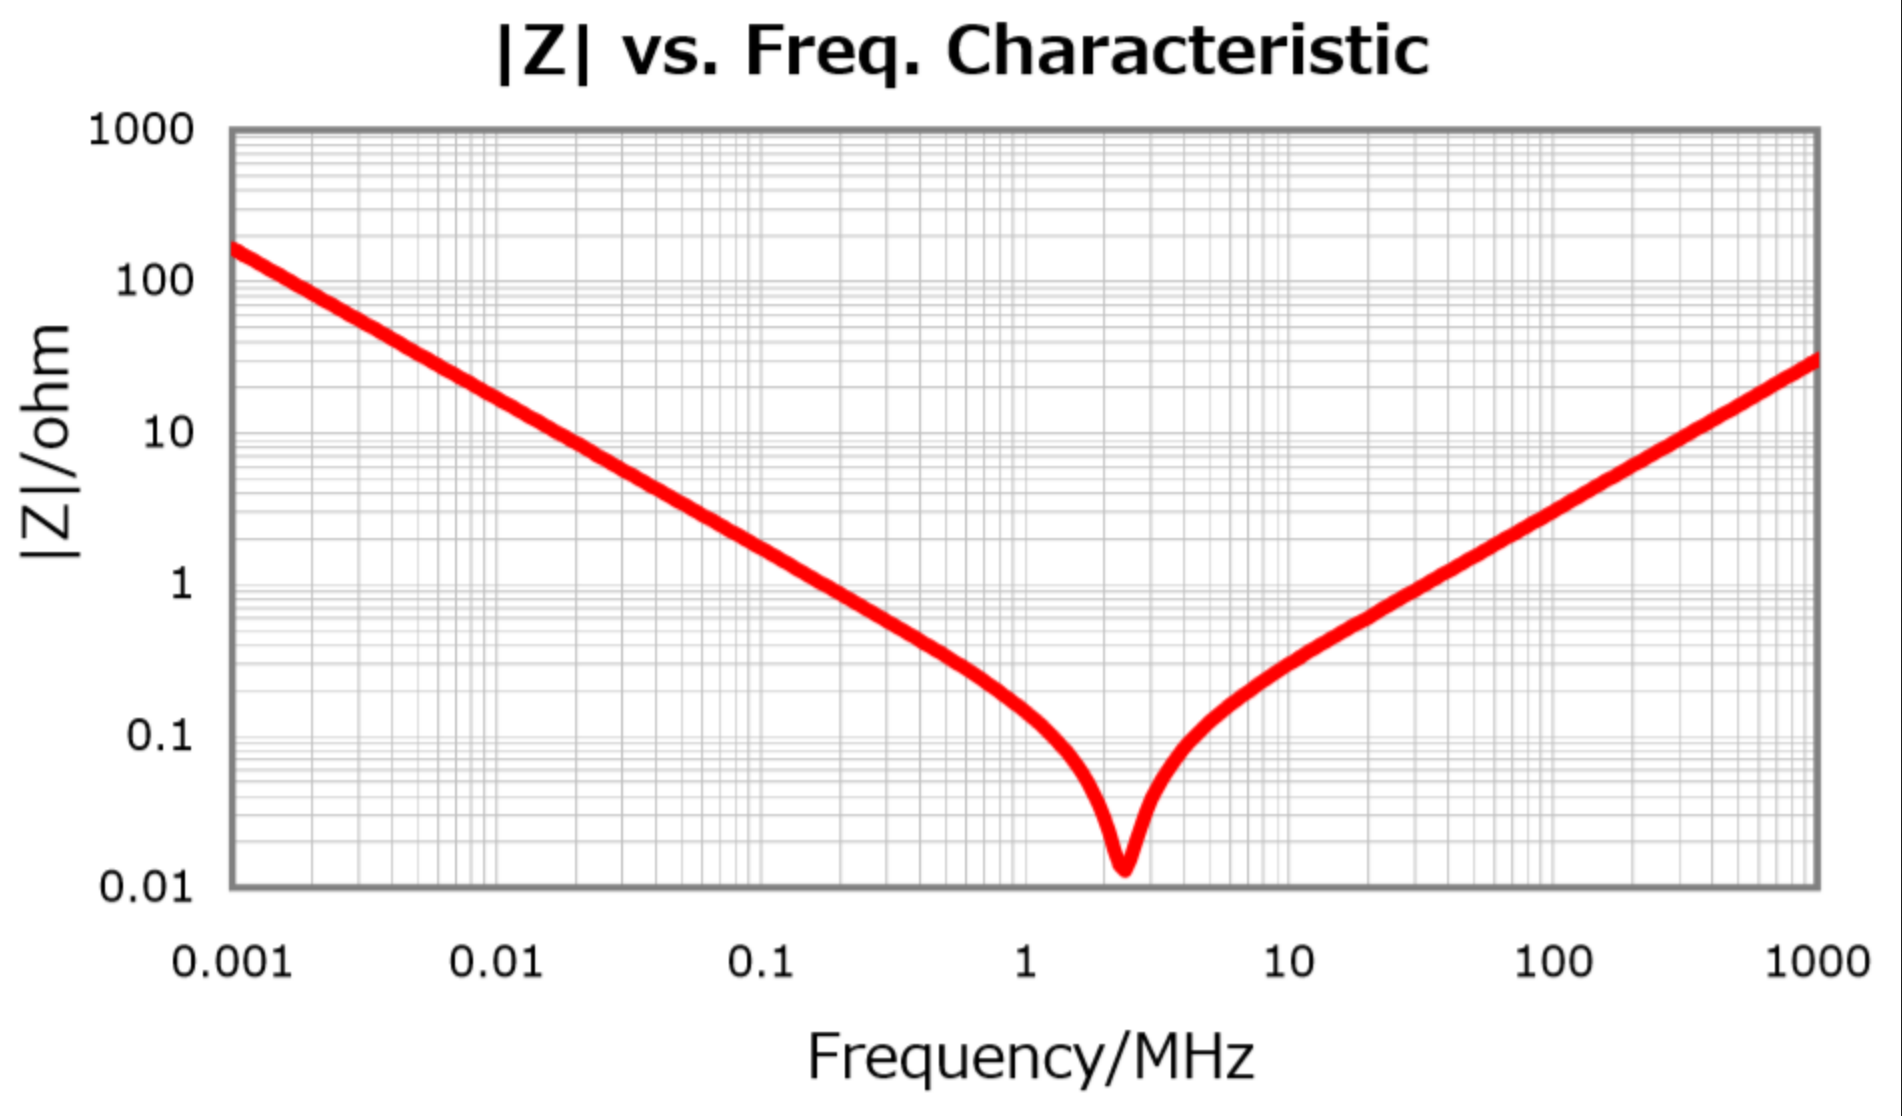
\includegraphics[scale=0.1]{../figures/elec_cap.png}
\end{center}

Preferiamo quindi usare condensatori \textit{ceramici} per la $C_2$, che hanno una risposta più lineare alle alte frequenze, ma vengono prodotti con valori di capacità molto minori (ordine del $10^{-12}$ (pico) Farad). Combinando gli effetti di un condensatore $C_1$ elettrolitico e di un $C_2$ ceramico, quindi, si riesce ad ottenere una rimozione del disturbo sia a bassa frequenza (da parte dell'elettrolitico) che ad alta frequenza (da parte del ceramico).

\subsubsection{Regolazione di corrente}
I regolatori di tensione lineare serie come li abbiamo trattati finora, quindi, sono largamente disponibili in commercio (ad esempio nella serie \textit{78xx} e \textit{79xx}, dove i 78 regolano tensione positiva e i 79 regolano tensione negativa).
Questi sono dotati di 3 terminali, $E$, $U$ ed $M$: 
\begin{center}
\begin{tikzpicture}[transform shape]
	% Paths, nodes and wires:
	\node[shape=rectangle, draw, line width=1pt, minimum width=2.965cm, minimum height=1.965cm] at (7.5, 6){} node[anchor=center, align=center, text width=2.577cm, inner sep=6pt] at (7.5, 6){78xx};
	\draw (11, 4) -- (7.5, 4) -| (7.5, 5);
	\draw (9, 6) -- (11, 6);
	\node[shape=rectangle, minimum width=0.465cm, minimum height=0.465cm] at (5.5, 6.5){} node[anchor=center, align=center, text width=0.077cm, inner sep=6pt] at (5.5, 6.5){E};
	\node[shape=rectangle, minimum width=0.465cm, minimum height=0.465cm] at (9.5, 6.5){} node[anchor=center, align=center, text width=0.077cm, inner sep=6pt] at (9.5, 6.5){U};
	\node[shape=rectangle, minimum width=0.465cm, minimum height=0.465cm] at (7, 4.5){} node[anchor=center, align=center, text width=0.077cm, inner sep=6pt] at (7, 4.5){M};
	\draw (11, 6) to[open, v=$V_X$, voltage=american] (11, 4);
\end{tikzpicture}
\end{center}
dove:
\begin{itemize}
	\item $U$ è il voltaggio di ingresso (cioè la $V_{in}$);
	\item $E$ è il voltaggio di uscita (cioè la $V_{out}$);
	\item $M$ è il ground (da \textit{Massa}).
\end{itemize}

Solitamente, questi dispositivi vengono usati per regolare la tensione, ma possono essere configurati anche per regolare la \textit{corrente}.
Il circuito, in particolare, è il seguente:
\begin{center}
\begin{tikzpicture}[transform shape]
	% Paths, nodes and wires:
	\node[shape=rectangle, draw, line width=1pt, minimum width=2.965cm, minimum height=1.965cm] at (7.5, 6){} node[anchor=center, align=center, text width=2.577cm, inner sep=6pt] at (7.5, 6){78xx};
	\draw (4, 4) to[battery1, l={$V_{cc}$}] (4, 2);
	\draw (4, 6) to[american voltage source, l={$V_S(t)r$}] (4, 4);
	\draw (11, 6) to[american resistor, l={$R$}] (11, 4);
	\draw (11, 4) to[american resistor, l={$R_L$}] (11, 2);
	\draw (11, 2) |- (4, 2);
	\draw (11, 4) -- (7.5, 4) -| (7.5, 5);
	\draw (9, 6) -- (11, 6);
	\draw (4, 6) -- (6, 6);
	\node[shape=rectangle, minimum width=0.465cm, minimum height=0.465cm] at (5.5, 6.5){} node[anchor=center, align=center, text width=0.077cm, inner sep=6pt] at (5.5, 6.5){E};
	\node[shape=rectangle, minimum width=0.465cm, minimum height=0.465cm] at (9.5, 6.5){} node[anchor=center, align=center, text width=0.077cm, inner sep=6pt] at (9.5, 6.5){U};
	\node[shape=rectangle, minimum width=0.465cm, minimum height=0.465cm] at (7, 4.5){} node[anchor=center, align=center, text width=0.077cm, inner sep=6pt] at (7, 4.5){M};
\end{tikzpicture}
\end{center}

La corrente sulla resistenza $I_R$ sarà data dalla tensione $V_X$ imposta dal \textit{78xx}:
$$
I_R = \frac{V_X}{R}
$$
per cui la corrente al carico sarà:
$$
I_L = I_R + I_M
$$
dove $I_m$ è solitamente nell'ordine dell milliampere. Questo significa che, se $I_R >> I_M$ (come abbiamo detto è effettivamente il caso), la corrente che imponiamo al carico sarà:
$$
I_L = I_R = \frac{V_X}{R}
$$
cioè siamo riusciti ad utilizzare il regolatore di tensione come regolatore di corrente.

Vediamo però che nella pratica questa configurazione non funzionerà sempre. Infatti, presupposto per il funzionamento del regolatore di tensione è che:
$$
V_E > V_U
$$
e anzi, che esista una certa \textit{caduta minima}, detta \textit{drop-out}:
$$
\mathrm{min} \left(V_E - V_U\right) = V_{\text{drop-out}}
$$
Il voltaggio di drop-out è solitamente nell'ordine del volt.
Ora, riprendendo il circuito a reoglatore di corrente, abbiamo che applicando la KVL sulla maglia esterna si ha:
$$
E_{DC} = V_{EU} + V_X + R_L I_L \implies V_{EU} = E_{DC} - V_X - R_L I_L
$$
dove $E_{DC}$ è quanto imposto dall'alimentazione variabile a sinistra (cioè la somma $E_{DC} = V_{cc} + V_s(t)$), e $V_{EU}$ è la caduta sul regolatore di tensione che ci interessa imporre maggiore al drop-out:
$$
V_{EU} = E_{DC} - V_X - R_L I_L \geq V_{\text{drop-out}}
$$
Dovrà quindi essere che la $R_L$ non è abbastanza grande da ridurre la caduta $V_{EU}$ al punto da portare il regolatore al di fuori del regime di operazione, cioè:
$$
R_L \leq \frac{E_{DC} - V_X - V_{\text{drop-out}}}{\left(\frac{V_X}{R}\right)}
$$

\par\smallskip

Vediamo che il circuito a regolatore lineare serie visto finora ha dei difetti:
\begin{enumerate}
	\item Un difetto del circuito  è che è piuttosto limitante nelle sue configurazioni, cioè una volta progettato il circuito per una tensione $V_{out}$ fissa, non si può variare velocemente questa tensione senza riprogettare l'intero circuito;
	\item Inoltre, dobbiamo sempre fornire in ingresso al circuito una $V_{in}$ che sia $>> V_{out}$, altrimenti l'uscita è instabile e sicuramente non ideale;
	\item Infine, il circuito ha caratteristiche pessime per quanto riguarda la potenza dissipata. Infatti, col fatto che $V_{out} << V_{in}$, tutta la potenza in eccesso fornita da $V_{in}$ sarà dissipata sotto forma di calore (per fissare la tensione di riferimento e per alimentare il partitore in ingresso all'OP amp).
\end{enumerate}

\subsubsection{Regolatore a commutazione}
Vediamo allora un'altro tipo di regolatore di tensione, cioè il regolatore a \textbf{commutazione} (dall'inglese \textbf{switched-mode} \textit{power supply}).

Il vantaggio principale dei regolatori a commutazione è dato dal fatto che questi dissipano molta poca potenza. Questo è permesso dal fatto che il componente usato per regolare la corrente è un \textit{interruttore}. L'interruttore dissipa potenza quasi nulla, in quanto può essere:
\begin{itemize}
	\item Chiuso, cioè in cortocircuito e non dissipa potenza;
	\item Aperto, cioè rappresenta un circuito aperto e ugualmente non dissipa potenza.
\end{itemize}

\newpage

Consideriamo il semplice circuito composto da una sorgente costante $E$, fatta passare attraverso un interruttore su un carico $R_L$.
\begin{center}
\begin{tikzpicture}[transform shape]
	% Paths, nodes and wires:
	\draw (4, 6) to[battery1, l={$E$}] (4, 4);
	\draw (4, 6) to[switch] (7, 6);
	\draw (7, 6) to[american resistor, l_={$R_L$}] (7, 4);
	\draw (7, 4) -- (8, 4);
	\draw (7, 6) -- (8, 6);
	\draw (7, 4) |- (4, 4);
	\draw (8, 6) to[open, v=$V_u$, voltage=american] (8, 4);
\end{tikzpicture}
\end{center}

Alternando la tensione su $R_L$, attraverso l'interruttore, fra $0$ e il picco ad $E$, otteniamo un andamento ad onda quadra con periodo $T_S$. Variando il rapporto fra il tempo a $0$ e il tempo a $E$ sul periodo $T_S$, si riesce quindi a modulare il cosiddetto \textit{duty cycle} $D$ dell'onda quadra:
$$
D = \frac{T_{ON}}{T_S}
$$

\begin{center}
	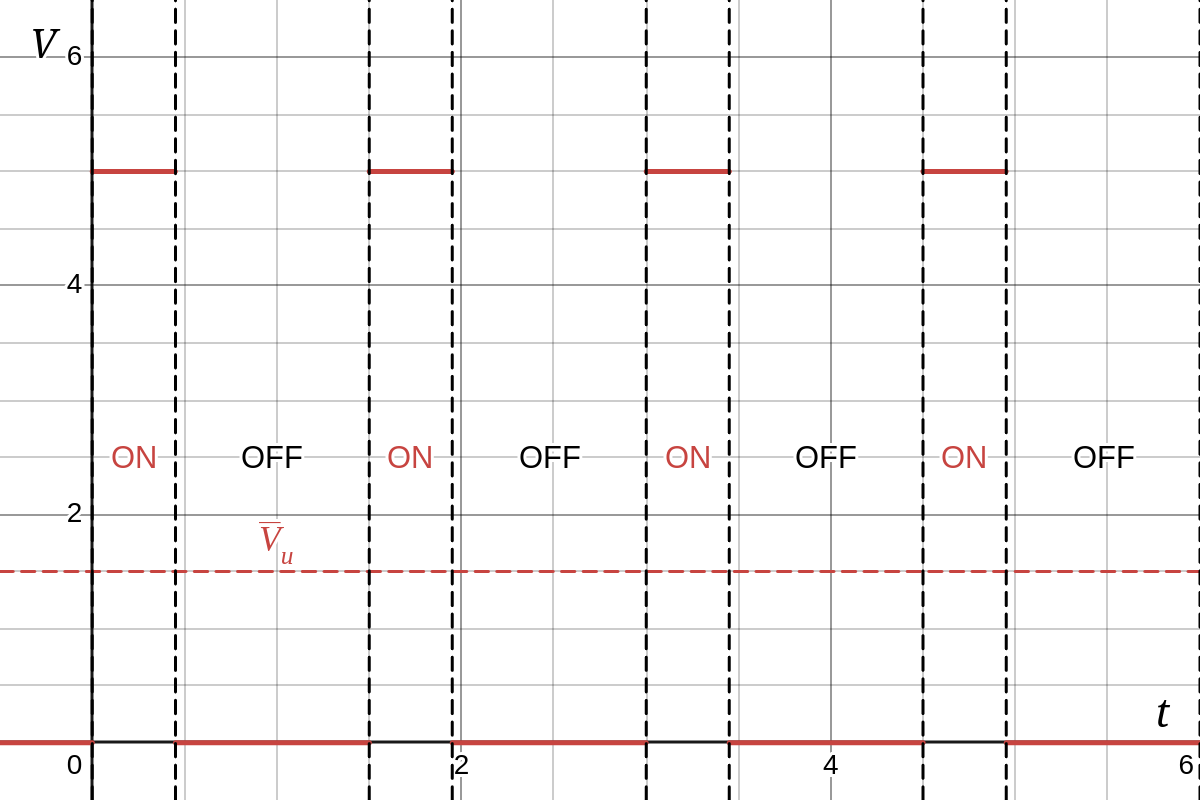
\includegraphics[scale=0.28]{../figures/switched_pwm.png}
\end{center}

Si scopre che il valore medio della $V_u$ in uscita sarà modulato proprio dal duty cycle, cioè varrà:
$$
\bar{V}_u = \frac{1}{T_S} \int_0^{T_S} V_u(t) \, dt = \frac{1}{T_S} E T_{ON} = ED
$$

La problematica a questo punto sarà che l'uscita $V_u$ dallo switch sarà altamente rumorosa (per le componenti ad alta frequenza date dalla commutazione continua in tensione). Dovremmo quindi mettere a valle del circuito un filtro passa basso, che isoli la componente DC e rimuova le componeGnte ad alta frequenza.
Il solito design del filtro passa basso passivo (cioè la rete RC) non è però adatto ai nostri scopi, in quanto nuovamente introdurremo una resistenza $R$ sulla maglia in potenza, quindi dissipando potenza e violando la specifica che ci eravamo imposti dall'inizio. 

\newpage

La soluzione consisterà nell'usare un filtro passa basso composto da solo condensatori ed induttanze anziché resistenze, cioè un filtro passa basso del \textit{secondo ordine}:
\begin{center}
\begin{tikzpicture}[transform shape]
	% Paths, nodes and wires:
	\draw (4, 6) to[battery1, l={$E$}] (4, 4);
	\draw (4, 6) to[switch] (7, 6);
	\draw (7, 4) |- (4, 4);
	\draw (7, 6) to[cute inductor, l={$L$}] (9, 6);
	\draw (9, 6) to[capacitor, l={$C$}] (9, 4);
	\draw (7, 4) -- (9, 4);
	\draw (9, 4) -- (11, 4);
	\draw (9, 6) -- (11, 6);
	\draw (11, 6) to[american resistor, l={$R$}] (11, 4);
	\node[shape=rectangle, draw, line width=1pt, dash pattern={on 4pt off 4pt}, minimum width=3.215cm, minimum height=3.465cm] at (8.625, 5.2){};
	\node[shape=rectangle, minimum width=3.215cm, minimum height=0.465cm] at (8.625, 7.2){} node[anchor=center, align=center, text width=2.827cm, inner sep=6pt] at (8.625, 7.2){Filtro LP};
\end{tikzpicture}
\end{center}

Questo tipo di sistema è stato studiato (se non sotto forma di circuito) nei corsi di fondamenti di automatica, e può essere studiato anche con le metodologie di Laplace viste ad elettrotecnica. Si ricava che la frequenza di taglio $\omega_0$ è data da:
$$
\frac{1}{\sqrt{LC}}
$$
Scegliendo quindi $L$ e $C$ in modo che $\omega_0$ sia molto minore della frequenza di switching $f_S = \frac{1}{T_S}$, riusciamo ad eliminare il rumore dato dalla commutazione ed isolare solo la componente DC che ci interessa.

Un'ultima problematica che rimane nel nostro circuito è che l'induttanza non si comporta bene con l'interruttore. Infatti, ricordiamo che l'induttanza è un componente che immagazina energia sotto forma di campo magnetico, e si oppone di conseguenza alle variazioni di corrente. Usare il circuito così come lo abbiamo presentato porterà, a tensioni abbastanza alte, alla formazione di scariche sull'interruttore in fase di apertura dell'interruttore, in quanto l'induttanza vuole appunto mantenere la corrente costante.

Introduciamo allora un diodo, che permetta all'induttanza di scaricare quando il circuito è aperto:
\begin{center}
\begin{tikzpicture}[transform shape]
	% Paths, nodes and wires:
	\draw (4, 6) to[battery1, l={$E$}] (4, 4);
	\draw (4, 6) to[switch] (7, 6);
	\draw (7, 4) |- (4, 4);
	\draw (7, 6) to[cute inductor, l={$L$}] (9, 6);
	\draw (9, 6) to[capacitor, l={$C$}] (9, 4);
	\draw (7, 4) -- (9, 4);
	\draw (9, 4) -- (11, 4);
	\draw (9, 6) -- (11, 6);
	\draw (11, 6) to[american resistor, l={$R$}] (11, 4);
	\draw (6, 4) to[empty diode, l_={$D$}] (6, 6);
\end{tikzpicture}
\end{center}

Chiamiamo questo tipo di circuito \textbf{regolatore switching "forward"}, dove l'operazione di commutazione è svolta in 2 fasi:
\begin{enumerate}
	\item Una prima fase $T_{ON}$, dove l'interruttore è chiuso e stiamo alimentando il carico. In questo caso il diodo è in interdizione (in quanto si trova $E$ sul catodo, per cui $V_{AK}$ sicuramente minore di $V_\gamma$);
	\item Una seconda fase $T_{OFF}$, dove l'interruttore è aperto, il diodo è in conduzione è permette alla corrente di scorrere nello stesso verso, ritornando all'induttanza attraverso il diodo. Il diodo, in questa fase, è mantenuto in conduzione dall'induttanza e dal condensatore, e in particolare dall'induttanza che come abbiamo detto si oppone ai cambiamenti di corrente. 
\end{enumerate}

Soffermiamoci sulla tensione sull'induttanza $L$. In condizioni normali, questa oscillerà fra due valori, cioè $E - V_u$ e $- V_u$, rispettivamente nelle fasi $T_{ON}$ e $T_{OFF}$, con andamento periodico dettato dallo switching.

La corrente a regime sull'induttanza sarà data integrando questa tensione in variazione continua, cioè:
$$
i_L(t) = \frac{1}{L} \int_0^t V_L(\tau) \, d\tau
$$
e, appunto perche siamo a regime, dovrà valere:
$$
i_L(t) = i_L(t + T_S) = \frac{1}{L} \int_0^{t + T_S} V_L(\tau) \, d\tau =
\frac{1}{L} \int_0^t V_L(\tau) \, d\tau + \frac{1}{L} \int_t^{t + T_S} V_L(\tau) \, d\tau
$$
cioè abbiamo scoperto che:
$$
\frac{1}{L} \int_0^t V_L(\tau) \, d\tau = \frac{1}{L} \int_0^t V_L(\tau) \, d\tau + \frac{1}{L} \int_t^{t + T_S} V_L(\tau) \, d\tau \implies \frac{1}{L} \int_t^{t + T_S} V_L(\tau) \, d\tau = 0 
$$
Questo significherà che la tensione media sull'induttanza sarà nulla, e potremo dire:
$$
i_L(t) = \frac{1}{L} \left( (E - V_u) T_{ON} - V_u T_{OFF} \right) = 0
$$
sul periodo $T_S$, e di conseguenza:
$$
E T_{ON} - V_u T_{ON} - V_u T_S + V_u T_{ON} = 0 \implies V_u = E\frac{T_{ON}}{T_S} = ED
$$
notando che $T_{OFF} = T_S - T_{ON}$, cioè otteniamo la caratteristica che avevamo detto dall'inizio. Conseguenza diretta è che l'integrale della tensione sull'induttore in fase $T_{ON}$ equivale all'integrale della tensione sulla fase $T_{OFF}$. Vediamola su un grafico:
\begin{center}
	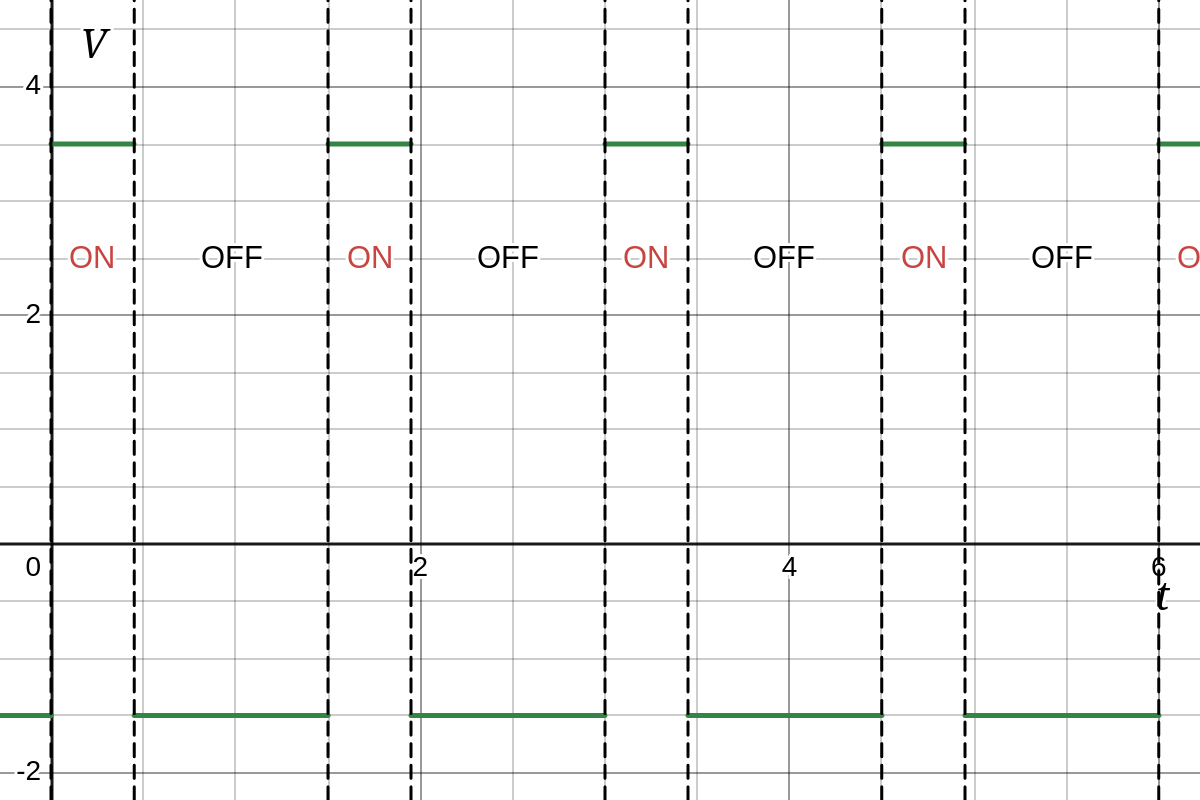
\includegraphics[scale=0.28]{../figures/inductor_pwm.png}
\end{center}

\end{document}
